\documentclass{article}
\setlength{\parskip}{0pt} % esp. entre parrafos
\setlength{\parindent}{20pt} % esp. al inicio de un parrafo
\usepackage{amsmath} % mates
\usepackage{listings}
\usepackage{xcolor}
\usepackage[sort&compress,numbers]{natbib} % referencias
\usepackage{url} % que las URLs se vean lindas
\usepackage[top=10mm,left=20mm,right=20mm,bottom=25mm]{geometry} % \textbf{\textbf{}}margenes
\usepackage{hyperref} % ligas de URLs
\usepackage{graphicx} % poner figuras
\usepackage{caption}
\usepackage{subcaption}
\usepackage[spanish]{babel} % otros idiomas
\hypersetup{
    colorlinks=true,
    linkcolor=blue,
    filecolor=blue,      
    urlcolor=blue,
}
\renewcommand{\lstlistingname}{C\'odigo}
\definecolor{codegreen}{rgb}{0,0.6,0}
\definecolor{codegray}{rgb}{0.5,0.5,0.5}
\definecolor{codepurple}{rgb}{0.58,0,0.82}
\definecolor{backcolour}{rgb}{0.95,0.95,0.92}
\lstdefinestyle{mystyle}{
    backgroundcolor=\color{backcolour},   
    commentstyle=\color{codegreen},
    keywordstyle=\color{magenta},
    numberstyle=\tiny\color{codegray},
    stringstyle=\color{codepurple},
    basicstyle=\ttfamily\footnotesize,
    breakatwhitespace=false,         
    breaklines=true,                 
    keepspaces=true,                 
    numbers=left,                    
    numbersep=5pt,                  
    showspaces=false,                
    showstringspaces=false,
    showtabs=false,                  
    tabsize=2
}
\lstset{style=mystyle}

\title{Reporte 8:\\Modelo de Urnas}
\author{Jorge Torres}
\date{\today}

\begin{document}

\maketitle

\section{Objetivo}\label{obj}
En esta pr\'actica se realiza la simulaci\'on de un sistema de coalescencia y fragmentaci\'on de part\'iculas, en donde una cantidad $n$ de part\'iculas forma inicialmente una cantidad $k$ de c\'umulos de diversos tama\~nos. En cada paso de la iteraci\'on, un c\'umulo puede unirse a otro o puede fragmentarse en dos c\'umulos m\'as peque\~nos, no necesariamente del mismo tama\~no. El objetivo consiste en estudiar estad\'isticamente el efecto que tiene la tasa $n/k$ en el porcentaje de part\'iculas que se lograr\'ian filtrar si se tuviese un filtro de un tama\~no determinado. En esta ocasi\'on, se utilizan tres cantidades de part\'iculas en combinaci\'on con tres cantidades de c\'umulos iniciales, dando un total de 9 combinaciones para la tasa $n/k$.

\section{Desarrollo}\label{des}
El desarrollo de la presente pr\'actica est\'a basado en el \href{https://github.com/satuelisa/Simulation/blob/master/UrnModel/aggrFrag.py}{c\'odigo} implementado por E. Schaeffer \cite{elisa1}, en donde realiza una simulaci\'on de uni\'on y fragmentaci\'on de part\'iculas. El \href{https://github.com/FeroxDeitas/Simulacion-Nano/blob/main/Tareas/P8/urnas.py}{desarrollo} completo puede encontrarse en el repositorio en GitHub de J. Torres \cite{jorge1}.\\

En primera instancia, se defninen los par\'ametros iniciales con los que opera la simulaci\'on. \'Estos consisten de una lista con las tres cantidades de c\'umulos iniciales, \texttt{clusters}; una lista con las tres cantidades de part\'iculas, \texttt{particles}; el tama\~no del filtro, en t\'erminos de la cantidad m\'inima de part\'iculas que debe tener un c\'umulo para que se quede alojado en el mismo, \texttt{filtersize}; la cantidad de iteraciones que se realizan para cada combinaci\'on de part\'iculas y c\'umulos, \texttt{runs}; y la cantidad de pasos que dura cada iteraci\'on para cada combinaci\'on, \texttt{dur}. Los par\'ametros se pueden ver implementados en el c\'odigo \ref{codigo1}.

\begin{lstlisting}[caption=Par\'ametros de Operaci\'on, label=codigo1, language=Python]
clusters = [2500, 5000, 10000]
particles = [250000, 500000, 1000000]
filtersize = 100
runs = 100
dur = 50
\end{lstlisting}

En el c\'odigo \ref{codigo2} se definen las probabilidades de que los c\'umulos se rompan o se unan con las funciones \texttt{rotura()} y \texttt{union()}, respectivamente. La probabilidad de rotura depende de manera sigmoidal de un tama\~no cr\'itico de c\'umulo, $c$, y de un factor arbitrario para suavizar la curva, $d$. El tama\~no cr\'itico est\'a dado por la media de tama\~nos de los c\'umulos en cada iteraci\'on, mientras que el factor de suavizaci\'on se determina con la desviaci\'on est\'andar de los tama\~nos de c\'umulos. Por otro lado, la probabilidad de uni\'on depende \'unicamente del tama\~no cr\'itico de manera exponencial negativa. De esta forma, los c\'umlos m\'as peque\~nos tienden a unirse, mientras que los m\'as grandes tienden a fracturarse.

\begin{lstlisting}[caption=Probabilidades de Rotura y Uni\'on, label=codigo2, language=Python]
def rotura(x, c, d):
    return 1 / (1 + exp((c - x) / d))
 
def union(x, c):
    return exp(-x / c)
    
c = np.median(cumulos)
d = np.std(cumulos) / 4
\end{lstlisting}

En seguida, en el c\'odigo \ref{codigo3} se definen las funciones \texttt{romperse()} y \texttt{unirse()}. La funci\'on \texttt{romperse()} decide qu\'e c\'umulos se romper\'an en el siguiente paso y qu\'e tama\~nos tendr\'an los dos c\'umulos resultantes de la rotura, mientras que la funci\'on \texttt{unirse()} crea dos grupos de c\'umulos para posteriormente decidir cu\'ales se unir\'an con cu\'ales en el pr\'oximo paso de la iteraci\'on. Estas funciones dependen respectivamente de las probabilidades de rotura y uni\'on descritas en el c\'odigo \ref{codigo2}.

\begin{lstlisting}[caption=Acciones de Rotura y Uni\'on de C\'umulos, label=codigo3, language=Python]
def romperse(tam, cuantos):
    if tam == 1:
        return [tam] * cuantos
    res = []
    for cumulo in range(cuantos):
        if random() < rotura(tam, c, d):
            primera = randint(1, tam - 1)
            segunda = tam - primera
            assert primera > 0
            assert segunda > 0
            assert primera + segunda == tam
            res += [primera, segunda]
        else:
            res.append(tam)
    assert sum(res) == tam * cuantos
    return res
 
def unirse(tam, cuantos):
    res = []
    for cumulo in range(cuantos):
        if random() < union(tam, c):
            res.append(-tam)
        else:
            res.append(tam)
    return res
\end{lstlisting}

El siguiente paso, observado en el c\'odigo \ref{codigo4}, es comenzar la iteraci\'on entre las cantidades iniciales de c\'umulos y las cantidades de part\'iculas. Tambi\'en se comienzan las 100 repeticiones de cada combinaci\'on. Para cada repetici\'on se crea nuevamente una cantidad $k$ de c\'umulos, de tal manera que la distribuci\'on de tama\~nos siguen una distribuci\'on normal, no existen c\'umulos vac\'ios, en total suman a la cantidad $n$ de part\'iculas y todos los tama\~nos son n\'umeros enteros.

\begin{lstlisting}[caption=Inicio de Iteraciones y Creaci\'on de C\'umulos, label=codigo4, language=Python]
for k in clusters:
    resultados = pd.DataFrame()
    for n in particles:
        filtrados = []
        for r in range(runs):
            filtro = 0
            orig = np.random.normal(size = k)
            cumulos = orig - min(orig)
            cumulos += 1
            cumulos = cumulos / sum(cumulos)
            cumulos *= n
            cumulos = np.round(cumulos).astype(int)
            diferencia = n - sum(cumulos)
            cambio = 1 if diferencia > 0 else -1
            while diferencia != 0:
                p = randint(0, k - 1)
                if cambio > 0 or (cambio < 0 and cumulos[p] > 0):
                    cumulos[p] += cambio
                    diferencia -= cambio
            assert all(cumulos != 0)
            assert sum(cumulos) == n
\end{lstlisting}

En el c\'odigo \ref{codigo5}, se inician los 50 pasos de la iteraci\'on, en donde los c\'umulos son agrupados por tama\~nos y la cantidad de c\'umulos que existen con esos tama\~nos. Es aqu\'i donde se comienzan a fracturar y unir los c\'umulos con las funciones definidas en el c\'odigo \ref{codigo3}. Para cada paso de la iteraci\'on, primero se decide qu\'e c\'umulos van a romperse y se rompen; despu\'es, se decide qu\'e cumulos van a unirse y se unen de manera aleatoria unos con otros. Estos pasos crean una nueva distribuci\'on de cantidades y tama\~nos de c\'umulos para cada paso de la iteraci\'on.

\newpage

\begin{lstlisting}[caption=Fractura y Uni\'on de C\'umulos en la Iteraci\'on, label=codigo5, language=Python]
            for paso in range(dur):
                assert sum(cumulos) == n
                assert all([c > 0 for c in cumulos]) 
                (tams, freqs) = np.unique(cumulos, return_counts = True)
                cumulos = []
                assert len(tams) == len(freqs)
                for i in range(len(tams)):
                    cumulos += romperse(tams[i], freqs[i]) 
                assert sum(cumulos) == n
                assert all([c > 0 for c in cumulos]) 
                (tams, freqs) = np.unique(cumulos, return_counts = True)
                cumulos = []
                assert len(tams) == len(freqs)
                for i in range(len(tams)):
                    cumulos += unirse(tams[i], freqs[i])
                cumulos = np.asarray(cumulos)
                neg = cumulos < 0
                a = len(cumulos)
                juntarse = -1 * np.extract(neg, cumulos)
                cumulos = np.extract(~neg, cumulos).tolist()
                assert a == len(juntarse) + len(cumulos)
                nt = len(juntarse)
                if nt > 1:
                    shuffle(juntarse)
                j = juntarse.tolist()
                while len(j) > 1:
                    cumulos.append(j.pop(0) + j.pop(0))
                if len(j) > 0:
                    cumulos.append(j.pop(0))
                assert len(j) == 0
                assert sum(cumulos) == n
                assert all([c != 0 for c in cumulos])
\end{lstlisting}

Por \'ultimo, con el c\'odigo \ref{codigo6}, al final de cada iteraci\'on se decide la cantidad de c\'umulos que son lo suficientemente grandes para quedar en el filtro y se calcula un porcentaje de part\'iculas filtradas. Estos porcentajes se guardan en archivos que se utilizan para su posterior an\'alisis.

\begin{lstlisting}[caption=C\'alculo de Porcentajes de Part\'iculas Filtradas, label=codigo6, language=Python]
            for p in cumulos:
                if p >= filtersize:
                    filtro += 1
            porcentaje = (filtro / sum(cumulos)) * 100
            filtrados.append(porcentaje)

        resultados['n: ' + str(n) + ', k: ' + str(k)] = pd.DataFrame(filtrados)
    
    resultados.to_csv('urnas_{:d}.csv'.format(k))            
\end{lstlisting}

\section{Resultados}\label{res}

A manera de resultados, primero se muestra una visualizaci\'on de vi\~netas donde se observa el comportamiento a trav\'es del tiempo de una iteraci\'on de fracturas y uniones de c\'umulos por medio de histogramas. En segunda instancia, se muestran diagramas tipo viol\'in donde se relacionan la tasa de cantidad de part\'iculas a cantidad de c\'umulos iniciales, con el porcentaje de part\'iculas filtradas. Adem\'as, se explica el an\'alisis estad\'istico realizado para determinar si existe una diferencia estad\'isticamente significativa al variar la cantidad de c\'umulos iniciales.

\subsection{Comportamiento del Sistema a Trav\'es del Tiempo}

La figura \ref{fig1} muestra el comportamiento que tiene una iteraci\'on de la simulaci\'on a trav\'es del tiempo. Los par\'ametros de dicha iteraci\'on son una cantidad de part\'iculas, $n=250000$ y una cantidad inicial de c\'umulos, $k=2500$. Una visualizaci\'on animada de la misma iteraci\'on se puede encontrar en el archivo \href{https://github.com/FeroxDeitas/Simulacion-Nano/blob/main/Tareas/P8/urnas.gif}{GIF} del repositorio de J. Torres. Como se puede observar, el sistema tiende tener m\'as c\'umulos de tama\~nos cercanos al tama\~no cr\'itico, lo cual es de esperarse, ya que estar\'ian oscilando entre unirse y fracturarse.

\begin{figure}
     \begin{subfigure}[b]{0.49\textwidth}
         \centering
         \includegraphics[width=\textwidth]{Images/p8p_ct00.png}
         \caption{\ }
     \end{subfigure}
     \begin{subfigure}[b]{0.49\textwidth}
         \centering
         \includegraphics[width=\textwidth]{Images/p8p_ct09.png}
         \caption{\ }
     \end{subfigure}
     \begin{subfigure}[b]{0.49\textwidth}
         \centering
         \includegraphics[width=\textwidth]{Images/p8p_ct19.png}
         \caption{\ }
     \end{subfigure}
     \begin{subfigure}[b]{0.49\textwidth}
         \centering
         \includegraphics[width=\textwidth]{Images/p8p_ct29.png}
         \caption{\ }
     \end{subfigure}
     \begin{subfigure}[b]{0.49\textwidth}
         \centering
         \includegraphics[width=\textwidth]{Images/p8p_ct39.png}
         \caption{\ }
     \end{subfigure}
     \begin{subfigure}[b]{0.49\textwidth}
         \centering
         \includegraphics[width=\textwidth]{Images/p8p_ct49.png}
         \caption{\ }
     \end{subfigure}
     \caption{Evoluci\'on del sistema a trav\'es del tiempo}
     \label{fig1}
\end{figure}

\newpage

\subsection{An\'alisis Estad\'istico}
La figura \ref{fig2} muestra los diagramas tipo viol\'in de las nueve combinaciones entre cantidad de part\'iculas y cantidad inicial de c\'umulos, donde se observan las distribuciones del porcentaje de part\'iculas filtradas para las 100 iteraciones de cada combinaci\'on. En la figura \ref{fig2.1} se observan los porcentajes para la variaci\'on de cantidad de part\'iculas con una $k=2500$, para la figura \ref{fig2.2} la cantidad inicial de c\'umulos es $k=5000$, y para la figura \ref{fig2.3} es de $k=10000$.\\

Adem\'as de los diagramas tipo viol\'in, se realiz\'o un an\'alisis de varianza para determinar si existe una diferencia significativa al variar la cantidad de part\'iculas con las que trabaja el sistema. Del an\'alisis se encontr\'o que los porcentajes de part\'iculas filtradas no pertenecen a la misma distribuci\'on al variar la cantidad de part\'iculas, ya que los valores $p$ son mucho menores al valor de $0.05$ que es necesario para deducir lo contrario. Cabe mencionar que no se realiz\'o un an\'alisis para demostrar si los porcentajes pertenecen a la misma distribuci\'on al variar la cantidad inicial de c\'umulos formados. Sin embargo, al observar los diagramas se puede apreciar una diferencia considerable en las distribuciones, lo cual podr\'ia indicar que tambi\'en existe una relaci\'on entre el porcentaje de partt\'iculas filtradas y la cantidad inicial de c\'umulos.

\begin{figure}
\centering
    \begin{subfigure}[b]{0.49\textwidth}
         \centering
         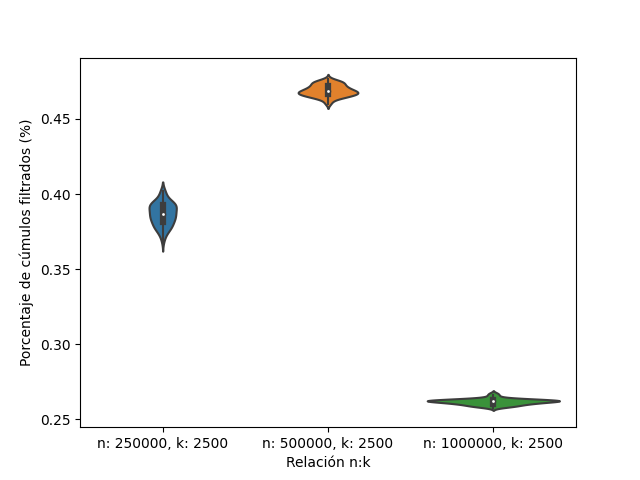
\includegraphics[width=\textwidth]{Images/Porcentajes_2500.png}
         \caption{Cantidad inicial de c\'umulos, $k=2500$}
         \label{fig2.1}
    \end{subfigure}
    \begin{subfigure}[b]{0.49\textwidth}
         \centering
         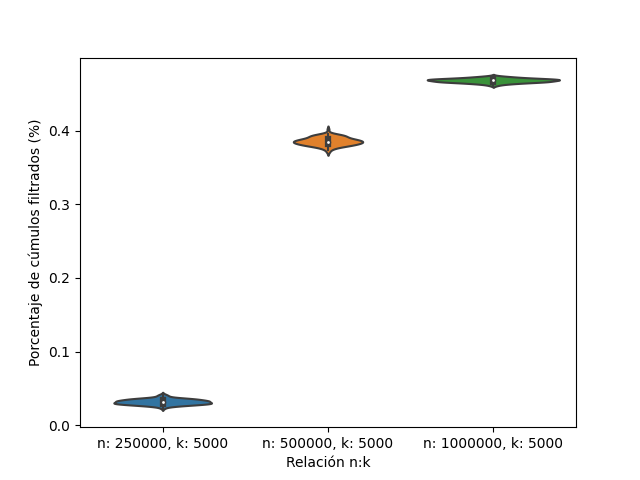
\includegraphics[width=\textwidth]{Images/Porcentajes_5000.png}
         \caption{Cantidad inicial de c\'umulos, $k=5000$}
         \label{fig2.2}
    \end{subfigure}
    \begin{subfigure}[b]{0.49\textwidth}
         \centering
         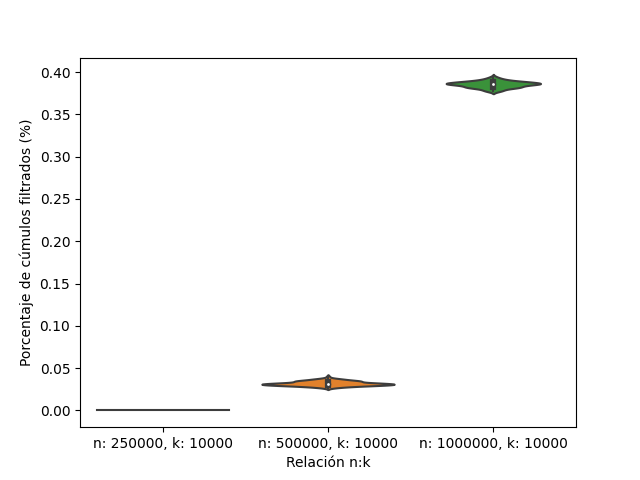
\includegraphics[width=\textwidth]{Images/Porcentajes_10000.png}
         \caption{Cantidad inicial de c\'umulos, $k=10000$}
         \label{fig2.3}
    \end{subfigure}
    \caption{Distribuci\'on de porcentajes de part\'iculas filtradas para cada tasa $n/k$.}
    \label{fig2}
\end{figure}

\section{Conclusiones}\label{con}
En la pr\'actica se realiz\'o la variaci\'on de la tasa entre cantidad de part\'iculas y cantidad inicial de c\'umulos, $n/k$, para determinar si existe una relaci\'on entre ella y el porcentaje de part\'iculas filtradas. Del an\'alisis estad\'istico se observa que hay una diferencia significativa al variar la cantidad de part\'iculas, por lo que es muy probable que exista una relaci\'on con la misma. Aunque no se realiz\'o el an\'alisis para determinar si tambi\'en hay relaci\'on con la cantidad inicial de c\'umulos, es f\'acil deducir que s\'i la hay al observar la gran diferencia de distribuciones de los diagramas tipo viol\'in.

\bibliography{tarea_8}
\bibliographystyle{plainnat}

\end{document}
